\section{Question}
The Cognitive Reflection Test (CRT) asks questions with a tempting wrong answer, the lure \citep{frederick2005cognitive}.
In dual-process accounts \citep{kahneman2011thinking,evans2013dualprocess}, a fast process proposes the lure and a slower process may notice the conflict and correct it \citep{pennycook2015what,deneys2012bias}.
Current language models offer two handles that loosely mirror this split.
Hidden reasoning can be switched off or on, and some models decide per call whether to reason \citep{fang2025thinkless}, reporting the number of reasoning tokens they spent.
Language models are often run as participants in cognitive experiments \citep{binz2025centaur}, including on the CRT \citep{binz2023using,hagendorff2023humanlike,yax2024studying}.
We observe only the reported reasoning tokens and the final answer.
We do not claim that they measure conflict detection, or that reported reasoning is a faithful account of how an answer was produced \citep{turpin2023language,chen2025reasoning}.

The famous CRT items circulate widely, so a model may answer them from memory.
Edited items on which the familiar procedure no longer works have been used to probe this kind of recitation \citep{yan2025recitation,xie2025grasp}.
We call an edited item a trap when the edit changes which procedure is valid, and pair each trap with a control that puts different words into the same slot and keeps the familiar procedure valid (Figure~\ref{fig:concept}).
On a trap, the familiar procedure gives a wrong answer, which we call the method answer.

\begin{figure}[t]
\centering
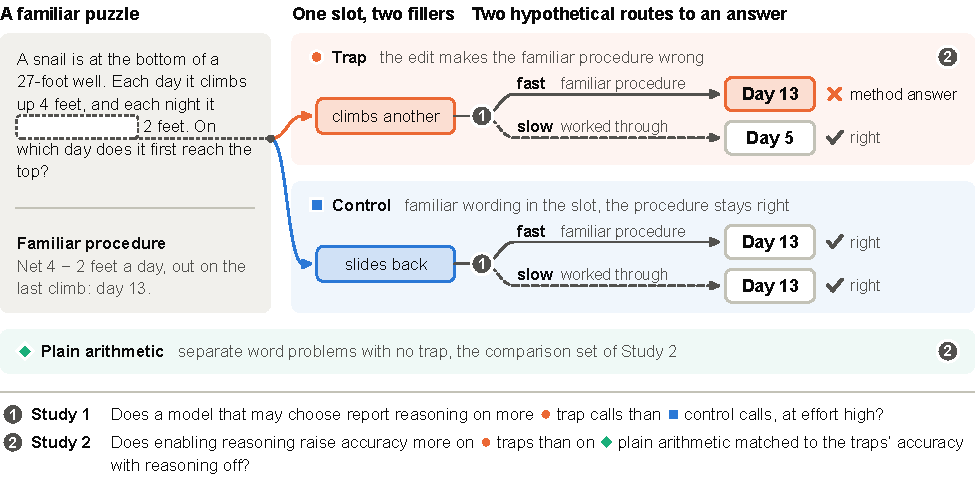
\includegraphics[width=\textwidth]{fig-concept}
\caption{The idea of both studies on one snail item in famous wording; the figure reports no result.
Trap and control fill the same slot of a familiar puzzle and share every number.
In the snail family the control keeps the familiar words, so only the trap changes the problem; in the other two families the control changes the slot as well.
The two routes are hypothetical and drawn only to explain the design.
The chips are worked answers, not model replies.
The familiar procedure gives day 13 on both items, and working the problem through gives day 5 on the trap and day 13 on the control.
The badges mark what each study compares.}
\label{fig:concept}
\end{figure}

Two questions follow.
Study 1 asks whether models that may choose report reasoning on more trap calls than control calls, and whether they reason more where reasoning raises accuracy.
Study 2 asks whether enabling reasoning raises the log-odds of accuracy more on traps than on plain arithmetic problems reweighted to the traps' accuracy with reasoning off.
Both studies were pre-specified.
Hypotheses, decision rules and analysis code were fixed before the first main-study call, and analyses labelled post hoc were added afterwards.
